\documentclass{scrartcl}
\usepackage[utf8]{inputenc}
\usepackage{listings}
\usepackage{geometry}
\usepackage[T1]{fontenc}
\usepackage{appendix}
\usepackage{graphicx}
\usepackage{amsthm}
\usepackage{amssymb}
\usepackage{amsmath}
\usepackage{mathtools}
\usepackage{float}
\usepackage[UKenglish]{babel}
\usepackage{url}
\usepackage{titling}
\usepackage{multirow}
\usepackage{subcaption}

\usepackage{algorithm}
\usepackage[noend]{algpseudocode}
\usepackage{amsfonts}

\DeclarePairedDelimiter\ceil{\lceil}{\rceil}
\DeclarePairedDelimiter\floor{\lfloor}{\rfloor}
\DeclareMathOperator{\Tr}{Tr}
\DeclareMathOperator{\sup}{sup}
\DeclareMathOperator{\inf}{inf}
\DeclareMathOperator*{\argmin}{\arg\!\min}
\DeclareMathOperator*{\argmax}{\arg\!\max}

\title{Computational Statistics\\Project Report}
%\author{...}

\begin{document}

    \maketitle


    \section{Introduction}
    In diesem Projekt reimplementiere ich den vorgeschlagenen Markov Chain Monte Carlo (MCMC) Algorithmus aus dem Paper
    \cite{lau2019} und versuche die Ergebnisse der Experimente zu reproduzieren. Der untersuchte Paper baut auf dem
    \textit{Metropolis-Hastings} MCMC Algorithmus \cite{metropolis1953} auf. \cite{liu2000}
    Der source code unter MIT Lizenz zu diesem Projekt findet sich in dem GitHub repository
    \begin{align*}
        \texttt{github.com/rinkwitz/Adaptive\_Plateau\_MCMC}\,.
    \end{align*}


    \section{Adaptive Component-wise Multiple-Try Metropolis Algorithm} Der Kernalgorithmus
    des Papers \cite{lau2019} besteht aus einem MCMC Algorithmus der drei Eigenschaften erfüllt. Der Algorithmus schlägt
    beim sampling mehrere Vorschläge aus verschiedenen Plateauverteilungen vor. Dies passiert unabhängig für alle
    Komponenten eines samples. Die Plateauverteilungen adaptieren ihre Form in Abhängigkeit von der Frequenz der akzeptierten sample Vorschläge.

	\subsection{Plateau Proposal Distributions}
    Der MCMC Algorithmus in \cite{lau2019} verwendet zum sampling von Vorschlägen \textit{non-overlapping plateau proposal distributions}.
	Die dabei verwendete grundlegende probability distribution function $f$ ist eine Kombination einer uniform distribution
	mit exponentiell decaying tails. Dabei ist die Verteilung $f$ konstant um einen Mittelwert $\mu$ in dem abgeschlossenen Intervall $[\mu-\delta,\mu+\delta]$ mit $\delta > 0$.
	Ausserhalb dieses Intervall folgt die Verteilung einem exponentiellen Verfall dessen tail Breite durch ein seitenabhängiges $\sigma_i >0$ bestimmt wird,
	je nachdem ob man sich auf der linken oder rechten Seite des Intervalls $[\mu-\delta,\mu+\delta]$ befindet. Definiert man
	eine unnormalisierte Verteilungsfunktion
	\begin{align*}
		\tilde{f}(y;\mu,\delta,\sigma_1,\sigma_2)&=\begin{cases}
			\exp\left( -\frac{1}{2\sigma_1^2}[y-(\mu-\delta)]^2 \right)&\quad ,y<\mu-\delta\\
           1&\quad ,\mu-\delta\leq y\leq\mu+\delta\\
           \exp\left( -\frac{1}{2\sigma_2^2}[y-(\mu+\delta)]^2 \right)&\quad ,y>\mu+\delta
		\end{cases}
	\end{align*}
    und berechnet das folgende Integral
    \begin{align*}
        C(\delta,\sigma_1,\sigma_2)&=\int\limits_{-\infty}^\infty\tilde{f}(y;\mu,\delta,\sigma_1,\sigma_2) dy\\
        &= \int\limits_{-\infty}^{\mu-\delta}\exp\left( -\frac{1}{2\sigma_1^2}[y-(\mu-\delta)]^2 \right)dy+
        \int\limits_{\mu-\delta}^{\mu+\delta}1dy+
        \int\limits_{\mu+\delta}^{\infty}\exp\left( -\frac{1}{2\sigma_2^2}[y-(\mu+\delta)]^2 \right)dy\\
        &=\frac{\sqrt{2\pi\sigma_1^2}}{2}+2\delta+\frac{\sqrt{2\pi\sigma_1^2}}{2}
    \end{align*}
    als die Summen von 2 halben Gausschen Integralen und einem Integral über eine konstatne Funktion, dann ergibt sich die normalisierte Verteilungsfunktion $f(y;\mu,\delta,\sigma_1,\sigma_2)=C(\delta,\sigma_1,\sigma_2)^{-1}\tilde{f}(y;\mu,\delta,\sigma_1,\sigma_2)$ \cite{lau2019}.
    Mithilfe von $f$ kann man die Plateau probability density distributions $T_{j,k}$, $j\in\{1,\dots,M\}$ für die trial proposals der $k$-ten Komponente definieren als
    \begin{align*}
        T_{j,k}(x,y)&=\begin{cases}
                          f(y;x,\delta_1,\sigma,\sigma)&,j=1\\
                          \frac 12 f(y;x-(2j-3)\delta-\delta_1,\delta,\sigma,\sigma)+\frac 12 f(y;x+(2j-3)\delta+\delta_1,\delta,\sigma,\sigma)&,j=2,\dots M-1\\
                          \frac 12 f(y;x-(2M-3)\delta-\delta_1,\delta,\sigma_0,\sigma)+\frac 12 f(y;x+(2M-3)\delta+\delta_1,\delta,\sigma,\sigma_1)&,j=M
        \end{cases}
    \end{align*}
    mit Werten $\delta_1,\delta,\sigma,\sigma_0,\sigma_1>0$. In Figure \ref{trial_proposals}
    sieht man die trial proposal propability density distributions für die Parameter $M=5, \delta_1=\delta=1,\sigma=0.05,\sigma_0=\sigma_1=0.5$. Man erkennt, dass sich die
    Verteilungen nur an ihren exponential decaying tails überschneiden. Die äußeren tails fallen durch die größeren $\sigma_0, \sigma_1$ Werte
    flacher ab als die restlichen tails. In dem Paper \cite{lau2019} verwenden die Autoren durchgehend die Werte $\delta=\delta_1=2,\sigma=0.05,\sigma_0=\sigma_1=3$.

    \begin{figure}
        \centering
        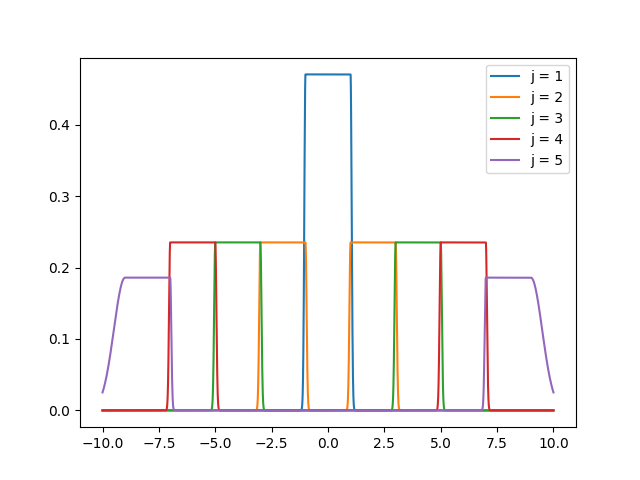
\includegraphics[scale=0.6]{../figs/fig_2b.png}
        \caption{Trial proposal propability density distributions for $M=5$}
        \label{trial_proposals}
    \end{figure}

    \subsection{Component-wise Multiple-Try Metropolis} Der \textit{Component-wise Multiple-Try Metropolis} Algorithmus,
    welcher die Grundlage für den Paper \cite{lau2019} bildet, startet mit seinem MCMC sampling Verfahren von einer Startposition
	$x_0\in\mathbb{R}^d$. Für jede MCMC Realisationen $x_n$ mit $n\in\{1,\dots,N\}$ wird für jede der $d$ Komponenten das folgende Verfahren
	angewendet. Sei $x=(x_1,\dots,x_d)$ der letzte gesampelte Kandidat des MCMC Algorithmus, dann schlägt der Algorithmus trials $z_j$
    für $i=1,\dots,M$ in dem er diese aus den Verteilungen $T_{j,k}(x_k,\cdot)$ sampelt. In meiner Reeimplementierung des Papers verwende
    ich dazu ein rejection sampling Verfahren \cite{rejection_sampling}. Dabei verwende ich eine gleichförmige Verteilung zum Erzeugen der samples über den folgenden Intervallen
%    \begin{itemize}
%        \item $j=1:I_1=[x_k-\delta_1-t_1,x_k+\delta_1+t_1]$ mit $t_1 = \sqrt{-2\sigma^2\log(0.0001C(\delta_1,\sigma,\sigma))}$,
%        \item $j=2,\dots,M-1:I_2=[x_k-2(j+1)\delta-\delta_1-t_2,x-2j\delta-\delta_1+t_2]\cup[x_k+2j\delta+\delta_1-t_2,x+2(j+1)\delta-\delta_1+t_2]$ mit $t_2=\sqrt{-2\sigma^2\log(0.0002C(\delta,\sigma,\sigma))}$, und
%        \item $j=M:I_3=[x_k-2(M+1)\delta-\delta_1-t_{32},x_k-2M\delta-\delta_1+t_{31}]\cup[x_k+2M\delta+\delta_1-t_{31},x_k+2(M+1)\delta+\delta_1+t_{32}]$ mit $t_{31}=\sqrt{-2\sigma^2\log(0.0002C(\delta,\sigma,\sigma_0))},t_{32}=\sqrt{-2\sigma_0^2\log(0.0002C(\delta,\sigma,\sigma_0))}$.
%    \end{itemize}
    \begin{align*}
        I_j = \begin{cases}
                  [x_k-\delta_1-t_1,x_k+\delta_1+t_1]\\\text{ for }j=1\text{ with }t_1 = \sqrt{-2\sigma^2\log(0.0001C(\delta_1,\sigma,\sigma))},\vspace{.25cm}\\
                  [x_k-2(j+1)\delta-\delta_1-t_2,x-2j\delta-\delta_1+t_2]\cup[x_k+2j\delta+\delta_1-t_2,x+2(j+1)\delta-\delta_1+t_2]\\\text{ for }j=2,\dots,M-1\text{ with }t_2=\sqrt{-2\sigma^2\log(0.0002C(\delta,\sigma,\sigma))},\text{ or}\vspace{.25cm}\\
                  [x_k-2(M+1)\delta-\delta_1-t_{32},x_k-2M\delta-\delta_1+t_{31}]\cup[x_k+2M\delta+\delta_1-t_{31},x_k+2(M+1)\delta+\delta_1+t_{32}]\\\text{ for }j=M\text{ with }t_{31}=\sqrt{-2\sigma^2\log(0.0002C(\delta,\sigma,\sigma_0))},t_{32}=\sqrt{-2\sigma_0^2\log(0.0002C(\delta,\sigma,\sigma_0))}.
        \end{cases}
    \end{align*}
    Diese Intervalle ermöglichen es in dem Bereich aus $T_{j,k}(x_k,\cdot)$ effektiv zu samplen wo die probability density function größer als $0.0001$ ist.
    Dazu sampelt man solange ein $u\sim U(0,1)$ und ein $y\sim U(I_i)$ bis
    \begin{align*}
        u < \frac{T_{j,k}(x_k,y)}{c|I_i|}
    \end{align*}
    erfüllt ist wobei $|I_j|$ die Breite des verwendeten Intervalls $I_j$ ist, $g_j$ die probability density function der gleichmäßigen Verteilung über $I_j$ ist und $c_j$ situationsabhängig folgende Werte hat
    \begin{itemize}
        \item $j=1:\quad c_1=\sup\limits_{y\in I_1}\frac{T_{1,k}(x_k,y)}{g_1(y)}=\frac{|I_1|}{C(\delta_1,\sigma,\sigma)}$,
        \item $j=2:\quad c_j=\sup\limits_{y\in I_j}\frac{T_{j,k}(x_k,y)}{g_j(y)}=\frac{|I_j|}{2C(\delta,\sigma,\sigma)}$, und
        \item $j=M:\quad c_M=\sup\limits_{y\in I_M}\frac{T_{M,k}(x_k,y)}{g_M(y)}=\frac{|I_M|}{2C(\delta,\sigma,\sigma_0)}$.
    \end{itemize}


    \subsection{Adaption of Proposal Distributions}
    TO DO ...


    \section{Experiments and Results}

    \subsection{Performance Measures}
    Die Autoren in dem Paper \cite{lau2019} verwenden zwei performance measures, um die Wirksamkeit des implementierten
    Algorithmus zu untersuchen. Dies ist zum einen die integrated autocorrelation times (ACT), welche in $R$ MCMC
    Simulationen mit jeweils $N$ Schritten für $K$ Komponenten berechnet wird. Sei im Folgenden
    $X_t^{(r)}=(X_{t,1}^{(r)},\dots,X_{t,K}^{(r)})$ das Ergebnis der $r$-ten MCMC Simulation bei Schritt $t$, wobei
    $r\in\{1,\dots,R\}$ und $t\in\{1,\dots,N\}$. Die Implementierung benutzt einen \textit{initial positive sequence estimator}
    wie ihn \cite{geyer1992} verwendet. Dafür wird zunächst die komponentenweise die empirische Autokovarianz bestimmt um
    die lagged autocovariance $\gamma_{i,k}^{(r)}$ mit $k\in\{1,\dots,K\}$ zu schätzen. Dabei ist
    \begin{align*}
        \hat{\gamma}_{t,k}^{(r)}&=\frac{1}{N}\sum\limits_{i=1}^{N-t}(X_{i,k}^{(r)}-\bar{X_k}^{(r)})(X_{i+t,k}^{(r)}-\bar{X_k}^{(r)})
    \end{align*}
    wobei $\bar{X_k}^{(r)}=1/N\sum\nolimits_{i=1}^NX_{i,k}^{(r)}$ das arithmetische Mittel $k$-ten Komponente in der $r$-ten
    Simulation bezeichnet. Danach schauen wir uns die Summen
    \begin{align*}
        \hat{\Gamma}_{m,k}^{(r)} &= \hat{\gamma}_{2m,k}^{(r)} + \hat{\gamma}_{2m+1,k}^{(r)}
    \end{align*}
    von benachbarten Autokovarianzen Paaren an. Schließlich ergibt sich die integrated autocorrelation times als
    \begin{align*}
        \text{ACT}_k^{(r)}&=-\hat{\gamma}_{0,k}^{(r)}+2\sum\limits_{i=0}^{m}\hat{\Gamma}_{m,k}^{(r)}
    \end{align*}
    wobei $m$ die größte natürliche Zahl ist, sodass $\hat{\Gamma}_{i,k}^{(r)} > 0$ für alle $i\in\{1,\dots,m\}$ gilt
    \cite{geyer1992}.

    \subsection{Experiments}
    TO DO ...

    \subsection{Technical Details of Implementation}
    TO DO ...

    \subsection{Results}
    Die zu den Experimenten zugehörigen Violinen plots findet man für die Zielverteilungen $\pi_1$, $\pi_2$, $\pi_3$ und $\pi_4$ finden sich
    in den Figures \ref{violin_plots_pi_1}, \ref{violin_plots_pi_2}, \ref{violin_plots_pi_3} und \ref{violin_plots_pi_4}. Dort findet man
    die komponenteweise Darstellung der ACT Werte in den Subfigures \ref{violin_plots_pi_1_act}, \ref{violin_plots_pi_2_act}, \ref{violin_plots_pi_3_act} und \ref{violin_plots_pi_1_act}, sowie
    die komponentenweise Darstellung der ASJD Werte in den Subfigures \ref{violin_plots_pi_1_asjd}, \ref{violin_plots_pi_2_asjd}, \ref{violin_plots_pi_3_asjd} und \ref{violin_plots_pi_4_asjd}.

    \begin{figure}
        \centering
        \begin{subfigure}{0.45\textheight}
              \centering
              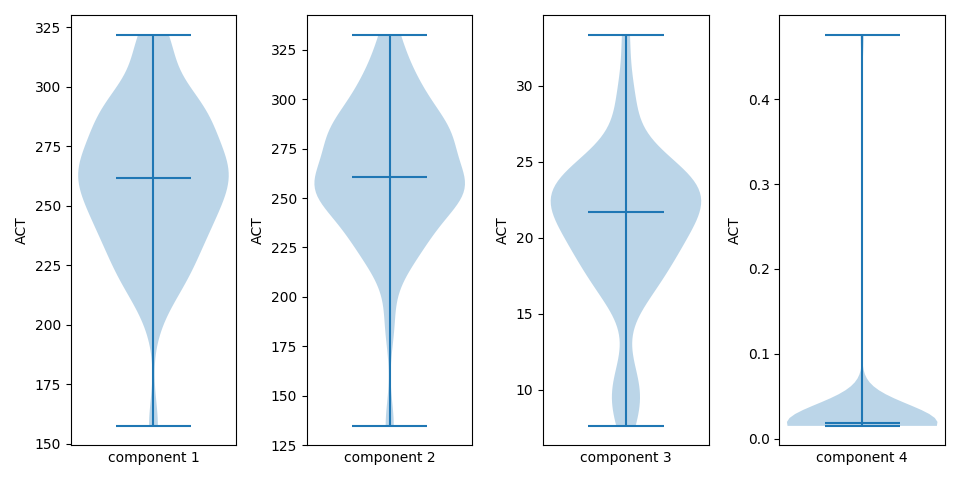
\includegraphics[width=.8\linewidth]{../figs/ACT_pi_1.png}
              \caption{komponenteweise ACT Werte für Zielverteilung $\pi_1$}
              \label{violin_plots_pi_1_act}
        \end{subfigure}
        \begin{subfigure}{0.45\textheight}
              \centering
              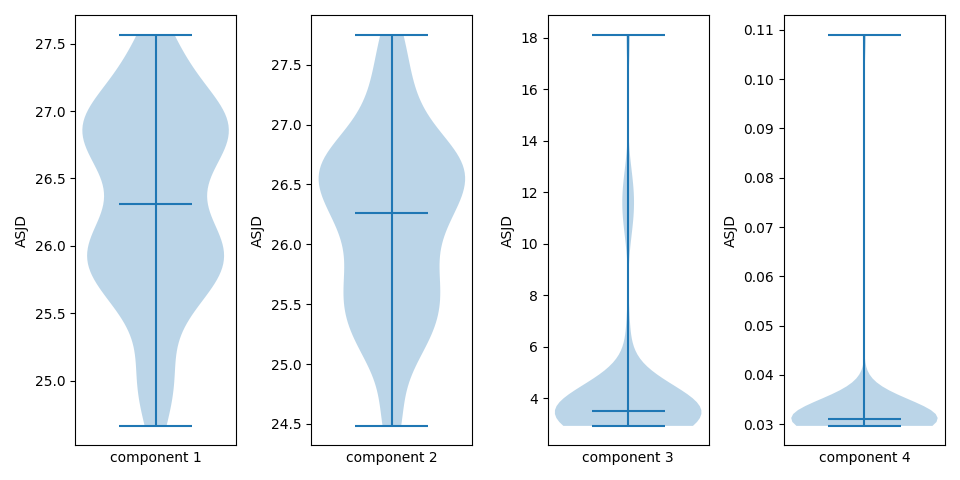
\includegraphics[width=.8\linewidth]{../figs/ASJD_pi_1.png}
              \caption{komponenteweise ASJD Werte für Zielverteilung $\pi_1$}
              \label{violin_plots_pi_1_asjd}
        \end{subfigure}
        \caption{Violin plots of performance measures for target distribution $\pi_1$}
        \label{violin_plots_pi_1}
    \end{figure}

    \begin{figure}
        \centering
        \begin{subfigure}{0.45\textheight}
              \centering
              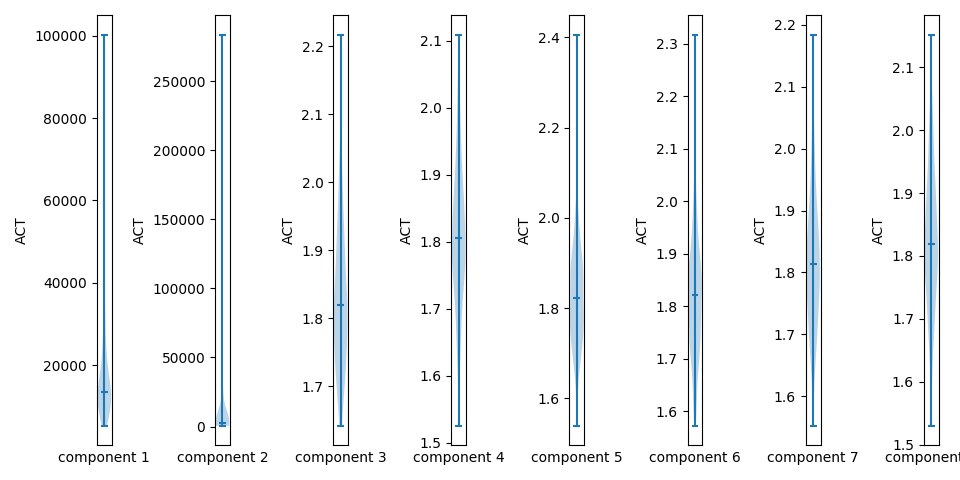
\includegraphics[width=.8\linewidth]{../figs/ACT_pi_2.png}
              \caption{komponenteweise ACT Werte für Zielverteilung $\pi_2$}
              \label{violin_plots_pi_2_act}
        \end{subfigure}
        \begin{subfigure}{0.45\textheight}
              \centering
              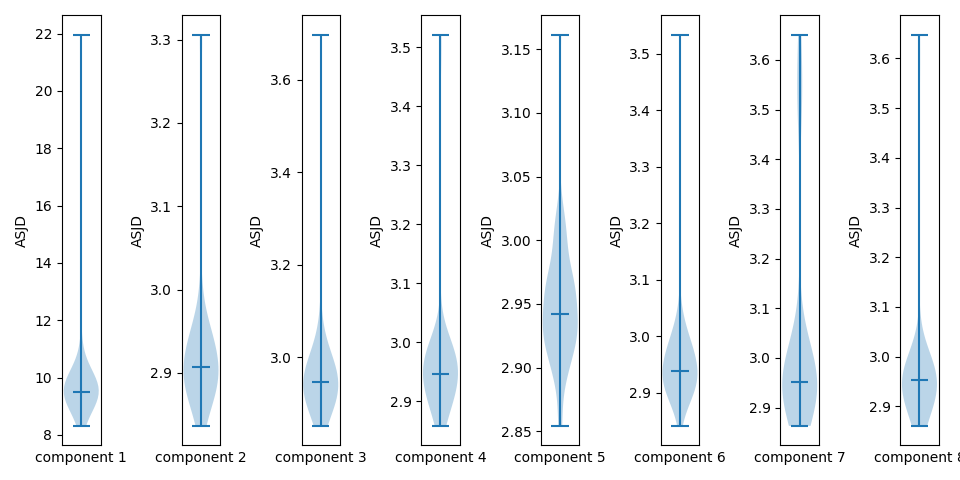
\includegraphics[width=.8\linewidth]{../figs/ASJD_pi_2.png}
              \caption{komponenteweise ASJD Werte für Zielverteilung $\pi_2$}
              \label{violin_plots_pi_2_asjd}
        \end{subfigure}
        \caption{Violin plots of performance measures for target distribution $\pi_2$}
        \label{violin_plots_pi_2}
    \end{figure}

    \begin{figure}
        \centering
        \begin{subfigure}{0.45\textheight}
              \centering
              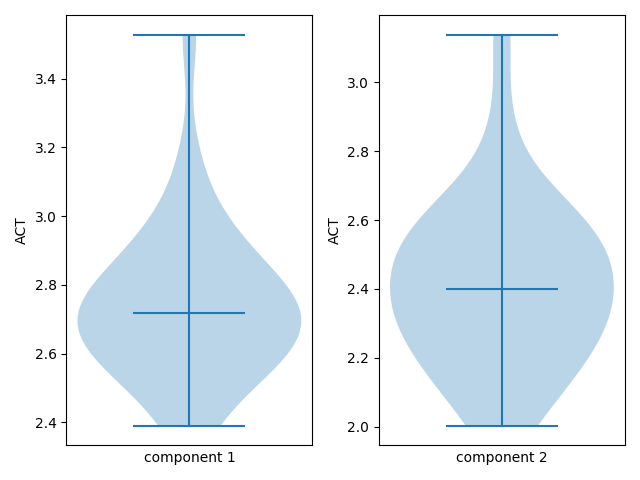
\includegraphics[width=.8\linewidth]{../figs/ACT_pi_3.png}
              \caption{komponenteweise ACT Werte für Zielverteilung $\pi_3$}
              \label{violin_plots_pi_3_act}
        \end{subfigure}
        \begin{subfigure}{0.45\textheight}
              \centering
              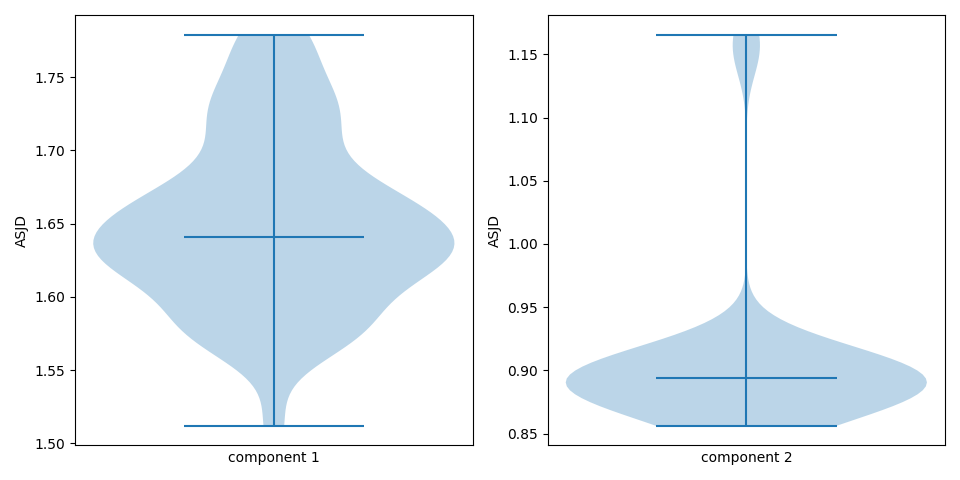
\includegraphics[width=.8\linewidth]{../figs/ASJD_pi_3.png}
              \caption{komponenteweise ASJD Werte für Zielverteilung $\pi_3$}
              \label{violin_plots_pi_3_asjd}
        \end{subfigure}
        \caption{Violin plots of performance measures for target distribution $\pi_3$}
        \label{violin_plots_pi_3}
    \end{figure}

    \begin{figure}
        \centering
        \begin{subfigure}{0.45\textheight}
              \centering
              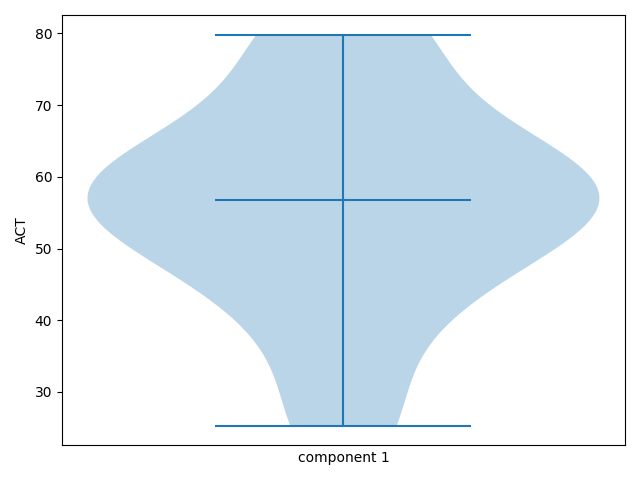
\includegraphics[width=.8\linewidth]{../figs/ACT_pi_4.png}
              \caption{komponenteweise ACT Werte für Zielverteilung $\pi_4$}
              \label{violin_plots_pi_4_act}
        \end{subfigure}
        \begin{subfigure}{0.45\textheight}
              \centering
              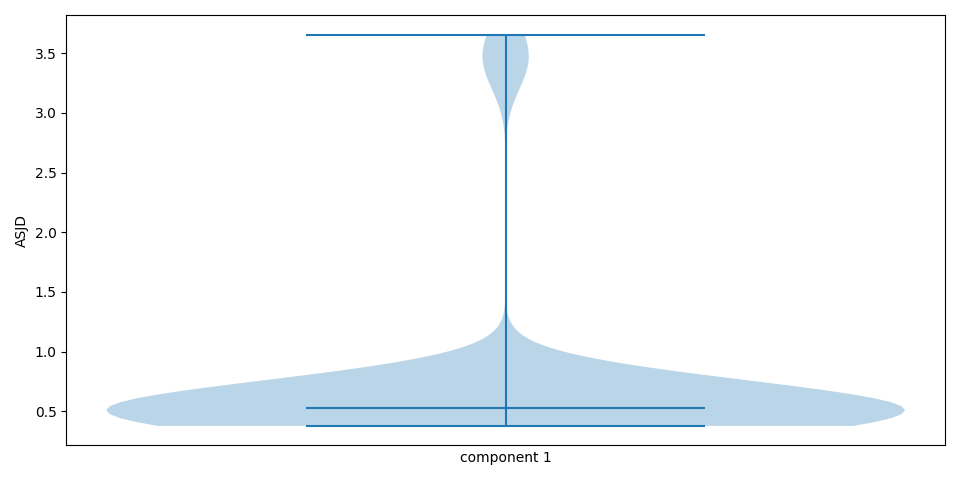
\includegraphics[width=.8\linewidth]{../figs/ASJD_pi_4.png}
              \caption{komponenteweise ASJD Werte für Zielverteilung $\pi_4$}
              \label{violin_plots_pi_4_asjd}
        \end{subfigure}
        \caption{Violin plots of performance measures for target distribution $\pi_4$}
        \label{violin_plots_pi_4}
    \end{figure}

    \section{Discussion}
    TO DO ...

    \bibliographystyle{apalike}
    \bibliography{ref}
\end{document}
